\subsection{Empfangseinheit}
\subsubsection{Tiefpass}
Die folgende Simulation(Abb. \ref{fig:frequencyResponse}) zeigt die Simulation des Butterworth-Tiefpasses durch FilterPro. Es sind der Frequenzgang(obere Kurve) und der Phasengang(untere Kurve) zu sehen. Der Tiefpass hat ab 100 Hz eine konstante Dämpfung von 60 dB je Dekade und zeigt damit das Verhalten eines Tiefpasses dritter Ordnung. Das zu übertragende Signal(50 Hz  Sinus) wird nicht gedämpft(0dB) und hat eine Phasenverschiebung von ca. $105^o$.
\begin{figure}[H]
\centering
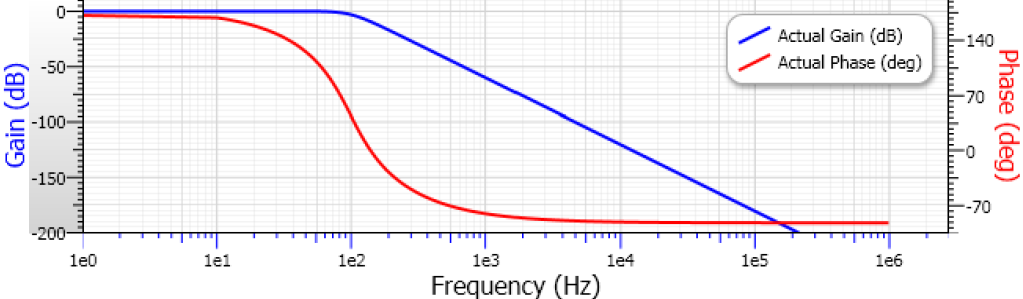
\includegraphics[scale=0.35]{gfx/simRx/FilterPro.png}
\caption{Simulation Frequenz-und Phasengang Butterworth-Tiefpass}
	\label{fig:frequencyResponse} 
\end{figure}


\subsubsection{Ausgangsverstärker}
Abbildung \ref{fig:amplifier} zeigt die Simulation der Verstärkung des Ausgangsverstärkers (Abschnitt \ref{sec:endamp}). Zur Simulation wurde ein Sinussignal von 100mV Amplitude und einer Frequenz von 50Hz eingeprägt. Das Potentiometer $"POTI"$(Abb. \ref{fig:endamp}) wurde mittels parametrischer Simulartion von $0 - 50k\Omega$ varriert und somit verschiedene Verstärkungsfaktoren von 0 bis 50 simuliert. Es ist zu erkennen, dass bei erreichen der Betriebsspannung der Verstärker clippt. 
\begin{figure}[H]
\centering
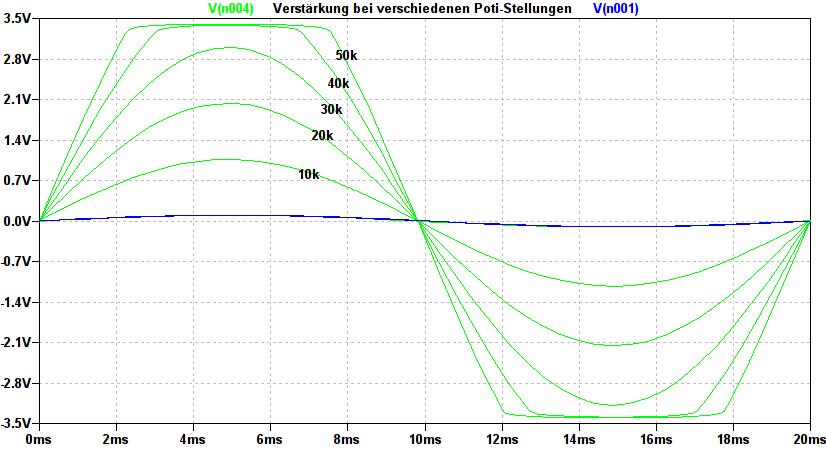
\includegraphics[scale=0.47]{gfx/simRx/amplification.png}
\caption{Simulation Ausgangsverstärker}
	\label{fig:amplifier} 
\end{figure}
